% Při kompilaci dokumentu LuaLaTeXem dojde k chybě, protože
% nedefinuje \pdfpagewidth a \pdfpageheight. 
% Balíček luatex85 to napravuje.
\RequirePackage{luatex85}
\PassOptionsToPackage{shorthands=off}{babel}
\makeatletter
\disable@package@load{fontenc}
\makeatother
\let\oldlooseness=\looseness
\documentclass{csbulletin}
\selectlanguage{czech}
\setcounter{secnumdepth}{3}
\usepackage{titlesec}
\titlelabel{\thetitle\enspace}
\usepackage{luavlna}
\usepackage[strict]{lua-widow-control}
\usepackage{csquotes}
\usepackage[
  backend=biber,
  style=iso-numeric,
  sortlocale=cs,
  autolang=other,
  bibencoding=UTF8,
  mincitenames=2,
  maxcitenames=2,
  isbn=false,
  shortnumeration=true,
]{biblatex}
\usepackage[version=4]{mhchem}
\usepackage{float}
\newfloat{listing}{htbp}{lop}
\floatname{listing}{Ukázka}
\def\lstfloatautorefname{Ukázka}
\renewcommand\multicitedelim{\addsemicolon\space}
\addbibresource{ruckert-profiling.bib}
\usepackage[implicit=false,hidelinks]{hyperref}

% Document commands [MR]
\font\niness=cmss10 at 9pt
\def\HiTeX{{\rm Hi\TeX}}
\def\HINT{{\niness H\kern.04em I\kern.04em NT\kern-.06em}}
\def\pdfTeX{{\rm pdf\kern 0.1em\TeX}}
\def\GUI{\acro{GUI}}
\def\WEB{{\tt WEB}}
\def\cweb{{\tt cweb}}
\def\texprof{{\tt texprof}}
\def\tprof{{\tt texprofile}}
\def\CEE{{\sc C}}
\def\Pascal{{\sc Pascal}}

\def\us{$\mu$\kern 0.5pt s}% micro seconds

\chardef\BS=`\\ % backslash in a string
\chardef\LB=`\{ % left brace in a string
\chardef\RB=`\} % right brace in a string
\chardef\UL=`\_ % underline character in a string
\chardef\HS=`\# % hash character in a string
\chardef\VB=`\| % vertical bar character in a string
\chardef\LQ=18  % left quote

\def\.#1{{\tt% simplified \verbatim
  \let\\=\BS % backslash in a string
  \let\{=\LB % left brace in a string
  \let\}=\RB % right brace in a string
  \let\_=\UL % underline in a string
  \let\#=\HS % hash in a string
  \let\|=\VB % hash in a string
  \let\`=\LQ % left quote
  #1\kern.05em}}

\def\ctl#1{{\tt\BS #1}}% for control sequences

% Document commands [VSN]
\ExplSyntaxOn
\newcommand
  \acro
  [ 1 ]
  {
    \tl_set:Nn
      \l_tmpa_tl
      { #1 }
    \regex_replace_all:nnN
      { [^\d]+ }
      { \c{textsc} \cB\{ \c{MakeLowercase} \cB\{ \0 \cE\} \cE\} }
      \l_tmpa_tl
    \regex_replace_all:nnN
      { \d+ }
      { \c{oldstylenums} \cB\{ \0 \cE\} }
      \l_tmpa_tl
    \tl_use:N
      \l_tmpa_tl
  }
\ExplSyntaxOff

\begin{document}

\singlechars{czech}{AaIiVvOoUuSsZzKk}

\title{Profilování \TeX ových dokumentů}
\EnglishTitle{Profiling \TeX{} Input Files}
\author{Martin Ruckert}
\podpis{Martin Ruckert\\
Hochschule München\\
Lothstrasse 64\\
80336 München\\
Germany\\
\url{martin.ruckert@hm.edu}}

\maketitle

\vspace{-10pt}

\begin{abstract}
Profiler je nástroj pro analýzu rychlosti kódu. Profiler může poskytovat informace o rychlosti jednotlivých řádků kódu nebo i celých procedur. Tyto informace jsou užitečné při optimalizaci kódu pro dosažení maximální rychlosti.

Ačkoliv jsou profilery běžně dostupné, doposud neexistoval profiler pro programátory, kteří připravují \TeX ová makra. V tomto článku představuji \texprof\ a \tprof: dva programy, které společně tvoří profiler pro \TeX ové dokumenty.
\end{abstract}
\klicovaslova: \TeX, profilování, \texprof, \tprof

\makeatletter
\def\@thefnmark{}\@footnotetext{Z~anglického originálu \cite{ruckert2024profiling} přeložil se svolením autora a vydavatele Vít Starý Novotný.}
\makeatother

\section{Kdo potřebuje profiler?}

\TeX ový profiler je nástroj pro programátory, kteří píšou makra pro \TeX. To však neznamená, že autor, který příležitostně napíše nějaké makro v \TeX u, by měl tento nástroj používat nebo že ho vůbec potřebuje. Optimalizace maker pro rychlost by měla být prováděna pouze tehdy, pokud se makro používá {\em velmi} často.

Abychom získali lepší představu, co znamená „{\em velmi} často“, provedeme následující úvahu: Za rozumných předpokladů\footnote{Spotřeba našeho počítače je 200 wattů a na kWh elektřiny připadá emise 500\,g \ce{CO2}.} vede jedna sekunda \acro{CPU} času k produkci 28\,mg \ce{CO2}. Opět za rozumných předpokladů\footnote{Spotřeba našeho vozu je 6\,l paliva na 100\,km a na litr paliva připadá emise 2370\,g \ce{CO2}.} způsobí jízda 200\,km emise 28\,kg \ce{CO2}. To znamená, že bychom museli ušetřit miliony sekund \acro{CPU} času, aby to mělo nějaký podstatný vliv na naši uhlíkovou stopu nebo rozpočet.

Příležitostní autoři \TeX ových maker mají lepší způsoby, jak trávit čas, než optimalizovat výkon. Existují ale oblíbené makrobalíčky s miliony uživatelů, jejichž makra se spouští mnohokrát za den. Pokud jsme autorem takového balíčku, možná nás zajímá, zda existují příležitosti k optimalizaci, kde tyto příležitosti v kódu hledat a jak velkého zrychlení můžeme docílit.

Možná ještě důležitější je, že profiler nám může říci, kde optimalizaci nehledat a zda změny v kódu přinesly požadovaný efekt. Obecně platí, že bychom nikdy neměli optimalizovat kód pro rychlost bez použití profileru.

\section{Jak funguje \TeX ový profiler?}

\subsection{Mapování příkazů na vstupní soubory a řádky}

\TeX ový stroj je interpretr, který čte vstupní soubory a vykonává vestavěné příkazy \TeX u, jako je například vytvoření horizontálního boxu, zvýšení hodnoty registru čítače nebo přidání znaku do aktuálního odstavce. \TeX ový profiler, nazvaný \texprof, je \TeX ový stroj s rozšířeními, která umožňují mapovat každý příkaz na vstupní soubor a na řádek v tomto souboru. K tomuto účelu využívá \texprof\ datové struktury, které si každý \TeX ový stroj (dále jen \TeX, pozn. překl.) udržuje, aby mohl zobrazovat užitečná hlášení v případě chyby.
Pokud je příkaz součástí formátového souboru, název vstupního souboru a číslo řádku nejsou známy. Dále se podíváme, jak se použití formátového souboru můžeme vyhnout.

I když se vyhneme použití formátového souboru, mnoho příkazů nepochází přímo ze vstupního souboru, ale z výsledku použití maker. Když definujeme makro, \TeX\ uloží příkazy z těla makra do tabulky. Když makro použijeme, \TeX\ načte z tabulky příkazy a vloží je na vstup. Jelikož jsou název vstupního souboru a číslo řádku známy během definice makra, může \texprof\ tyto informace také uložit do tabulky a načíst je spolu s příkazy při použití makra. Stejný mechanismus používá \texprof\ také v případě, že načítá vstup, například při hledání klíčového slova, a zjistí, že část příkazů musí vrátit na vstup pro pozdější zpracování. Tyto příkazy si s sebou také nesou informace o názvu vstupního souboru a čísle řádku.

Existuje několik vzácných případů, na které se výše uvedený mechanismus nevztahuje. \TeX\ např. vkládá složené závorky kolem výstupní rutiny, aby zajistil, že příkazy provedené ve výstupní rutině nezapříčiní neočekávané globální změny. Z pohledu \texprof u tyto složené závorky pochází z fiktivního řádku nula ve fiktivním vstupním souboru nazvaném ,,systém``.

Existují i další fiktivní čísla řádků ve fiktivním vstupním souboru ,,systém``, která \texprof\ používá. \TeX\ vyvolává systémové procedury, jako je rozdělení odstavce na řádky nebo zapsání stránky do souboru \acro{DVI}, které mohou být časově náročné. Bylo by zavádějící, kdybychom čas strávený v těchto rutinách přiřadili příkazu, který byl proveden na konci odstavce nebo způsobil zapsání stránky do souboru \acro{DVI}. Proto \texprof\ přiřazuje tyto časy k fiktivnímu souboru ,,systém`` a používá číslo řádku k označení odpovídající systémové procedury \TeX u.

\vspace{0.3cm}
\subsection{Mapování doby provádění příkazů}
Většina příkazů \TeX u se vykonává v proceduře \.{main\_control} \TeX u. V této proceduře najdeme smyčku, která čte příkazy a poté je vykonává pomocí kódu za návěštím \.{big\_switch} (dále jen ,,za \.{big\_switch}em``, pozn. překl.). Na začátku každé iterace této smyčky zaznamená \texprof\ čas z hardwarových hodin pomocí nízkoúrovňové rutiny operačního systému.

Zaznamenaný čas je začátkem nového časového intervalu a zároveň koncem předchozího časového intervalu. Po zaznamenání počátečního času \texprof\ pokračuje v běžném zpracování \TeX u a načte další příkaz ze vstupu. Jakmile je příkaz znám, \texprof\ zaznamená příkaz, vstupní soubor, číslo řádku (a také makro, ze kterého příkaz pochází; zaměříme se teď ale pouze na příkazy, makra budou vysvětlena později). Poté pokračuje běžné zpracování a příkaz je vykonán pomocí \.{big\_switch}e, který skončí návratem na začátek smyčky. Tam \texprof\ zaznamená koncový čas, vypočítá rozdíl a uloží příkaz, vstupní soubor, číslo řádku a časový rozdíl do velkého pole.

Občas je příkaz v \.{big\_switch}i nahrazen jiným příkazem a následně se \.{big\_switch} použije znovu k jeho vykonání. \texprof\ tuto výměnu ignoruje a zaznamená celý čas společně s příkazem, vstupním souborem a číslem řádku, které byly získány na začátku aktuální iterace. To do měření zavádí určitou nepřesnost, ale nezpůsobuje to výrazné chyby.

Mnohem větší vliv na přiřazení času souboru a řádku má existence hlavní smyčky \TeX u za návěštím \.{main\_loop}. Kód za návěštím \.{big\_switch} do této smyčky přejde vždy, když narazí na znak, a zůstane v ní, dokud čte příkazy typické pro běžný text: znaky, mezery, kerning, ligatury, změny písma a další podobné věci. Celý čas strávený v této smyčce je poté zaznamenán s příkazem, vstupním souborem a řádkem, které tuto smyčku zahájily. Čas potřebný ke zpracování celého odstavce tak může být přiřazen k prvnímu písmenu tohoto odstavce.
\oldlooseness=-1

Rozhodnutí nepřiřazovat čas přesněji je v tomto případě odůvodněno následujícími úvahami: Za prvé, takový odstavec je obvykle zpracován pouze jednou a doba zpracování obvykle nepředstavuje významnou část celkového běhu programu. Za druhé, při použití profileru nás obvykle nezajímá čas strávený nad písmeny, mezerami a dalšími částmi běžného textu. Koneckonců žádný autor neoptimalizuje text pro rychlost jeho zpracování. Toto rozhodnutí také výrazně snižuje počet časových intervalů, které musí \texprof\ zaznamenávat.

Procedura \.{main\_control} končí vykonáním příkazu \.{stop}, který zároveň ukončí zaznamenávání časových intervalů. Jako součást závěrečné procedury \TeX u \texprof\ zapíše všechna sesbíraná data do binárního souboru. Název tohoto souboru je získán připojením přípony \.{.tprof} k názvu vstupního souboru z vestavěného příkazu \ctl{jobname}. Další zpracování sesbíraných dat neprovádí \texprof, ale druhý program nazvaný \tprof. Jeho použití bude ilustrováno dále.

\subsection{Problém měření času}

Operační systémy obvykle poskytují několik hodin, ze kterých lze vybírat. \texprof\ používá \acro{POSIX}ovou funkci \.{clock\_gettime}, která měří \acro{CPU} čas aktuálního vlákna v nanosekundách. Ačkoliv nám čas v nanosekundách může připadat jako velmi přesný, skutečná přesnost je spíše v řádu stovek mikrosekund. To má několik důvodů, které si nyní popíšeme.

Moderní počítače provádí mnoho procesů současně a sdílí dostupná \acro{CPU} mezi prováděnými procesy, přičemž čas potřebný k přepnutí procesů zahrnuje zneplatnění obsahu keše. Instrukce pro načtení dat z hlavní paměti může trvat podstatně déle, pokud se daná paměťová oblast již nenachází v keši. Tento dodatečný čas je poté přiřazen k příkazu \TeX u, který se zrovna vykonává.

Moderní \acro{CPU} také používají techniku zvanou frekvenční škálování pro snížení spotřeby energie. Pokud jen píšeme text v editoru, může náš notebook běžet s frekvencí nižší než 1\,GHz. Krátce poté, co spustíte \TeX, si operační systém může všimnout, že je potřeba vykonat hodně práce, a může zvýšit frekvenci až na 4\,GHz. Všechny příkazy, které se vykonají po této změně, zaberou méně času než stejné příkazy před touto změnou.

V posledních letech začali výrobci kombinovat na jednom čipu několik výkonnostních jader s několika jádry úspornými. Zatímco výkonnostní jádra používají sofistikované superskalární pipeline pro vykonání více instrukcí v jednom cyklu, úsporná jádra používají jednoduché sekvenční provádění instrukcí, které sice spotřebuje podstatně méně energie a produkuje mnohem méně tepla, ale může potřebovat více cyklů na jednu instrukci.

Pokud se operační systém rozhodne přesunout \texprof\ z úsporného jádra na výkonnostní jádro uprostřed běhu, bude to mít drastický vliv na časy příkazů. Operační systém ho také může přesunout zpět na úsporné jádro, pokud \texprof\ začne provádět vstupně-výstupní operace a musí čekat na disk.

Existuje několik možností, jak tyto efekty zmírnit, například výpočtem průměru přes více běhů nebo použitím syntetických časů. Žádná z těchto metod však není momentálně implementována.

\vspace{-7.5pt}
\subsection{Mapování výpočetních časů na makra}
\label{tail-recursion}

Když \TeX\ narazí na aktivní znak nebo řídící sekvenci, ví, že musí vykonat primitivní příkaz nebo makro. U makra vyhledá seznam příkazů, které tvoří tělo makra, a tento seznam vloží na svůj zásobník vstupů. Když \TeX\ potřebuje další příkaz ze vstupu, vezme ho z nejvyššího seznamu na zásobníku. Jakmile \TeX\ dosáhne konce tohoto seznamu, odstraní ho ze zásobníku a pokračuje ve čtení příkazů ze seznamu pod ním.

Zásobník vstupů se nepoužívá pouze při použití maker, ale také pro implicitní volání jiných rutin \TeX u: Když je připravena nová stránka, konstruktor stránek vloží na zásobník vstupů výstupní rutinu. Na začátku odstavce systém vloží na zásobník příkazy z vestavěného příkazu \ctl{everypar}. Při použití vestavěného příkazu \ctl{input} se na zásobník vloží celé soubory. Je také běžné, že \TeX\ načítá vstup, například kvůli kontrole klíčového slova, a vloží nepoužité tokeny zpět na zásobník, pokud klíčové slovo nebylo nalezeno.

Většinu informací, které \texprof\ potřebuje ke sledování maker, lze nalézt na zásobníku vstupů \TeX u, ale ne všechny. Zásobník vstupů totiž neobsahuje informace o správné úrovni zanoření maker. Důvodem je chytrá optimalizace, kterou \TeX\ používá na svém zásobníku vstupů pro podporu koncové rekurze: Před vložením těla nového makra na zásobník \TeX\ opakovaně kontroluje, zda je nejvyšší seznam na zásobníku již prázdný. Pokud ano, odstraní prázdný seznam ze zásobníku. Teprve poté, co jsou všechny prázdné seznamy odstraněny, je tělo nového makra vloženo na zásobník.

Díky této optimalizaci může smyčka, která je implementována jako rekurzivní makro provádějící samo sebe jako poslední akci těla makra, běžet bez přetečení zásobníku. Bohužel tato technika odstraní makro ze zásobníku vstupů, zatímco jeho poslední podmakro stále běží, a nové makro se tak vloží na nižší úroveň zanoření, než je jeho skutečná úroveň zanoření.

Proto \texprof\ přidává informace o skutečné aktuální úrovni zanoření maker do zásobníku vstupů \TeX u a udržuje podpůrný zásobník, který obsahuje informace o všech makrech až po skutečnou úroveň zanoření: název makra, vstupní soubor a číslo řádku, kde bylo makro definováno. Tento podpůrný zásobník poskytuje informace o skutečném začátku a konci provádění makra, které jsou zaznamenávány společně s časovými údaji o vykonaných příkazech.

\section{Analýza profilovacích dat}

Surová data, která \texprof\ zapisuje do výstupního souboru, jsou jen dlouhý seznam tisíců záznamů ve formátu „příkaz, vstupní soubor, řádek, čas“ prokládaných záznamy, které odrážejí změny na zásobníku maker. Extrahování užitečných informací z těchto dat je úkolem samostatného programu nazvaného \tprof.

Pro vysvětlení použití \texprof u a \tprof ru je nejlepší použít skutečné příklady. Pro první příklad jsem hledal velký dokument zaměřený na text. Hledáním na internetu jsem našel \TeX ovou verzi Bible~\cite{allred2018bible}. Několika změnami jsem zajistil, že používá formát plain \TeX, takže využívá pouze omezené množství maker. Většina maker pochází z plain \TeX u, ale jsou zde také uživatelsky definovaná makra.

Spuštěním příkazu \.{texprof -prof bible} vznikne soubor \.{bible.tprof} o velikosti 17\,MB. Po spuštění příkazu \.{tprof bible} bez dalších voleb se zobrazí následující souhrn:

\begingroup
\medskip
\noindent
\centering
\begin{tabular}{@{}lr}
Celkový čas měření:          &    728,92\,ms\\
Celkový počet vzorků:        &   2\,157\,642\\
Průměrný čas na vzorek:      &    337,00\,ns\\
Celkový počet souborů:       &            69\\
Celkový počet maker:         &         1 097\\
Maximální hloubka zásobníku: &             7\\
\end{tabular}
\par
\medskip
\endgroup

\noindent
Pomocí dalších voleb můžeme specifikovat, které datové tabulky má \tprof\ zobrazit a jak by měl informace zobrazovat.

\subsection{Deset nejpomalejších řádků}

Při použití volby \.{-T} projde \tprof\ data, sečte časy pro každou kombinaci vstupního souboru a řádku, seřadí výsledky a zobrazí deset nejpomalejších řádků. Výstup příkazu \tprof\.{ -T bible} je zobrazen v Tabulce~\ref{bible-T}.

\begin{table}
\centering
\begin{tabular}{rrrrrrl}
soubor & řádek & procenta & čas [ms] & počet & průměr & soubor\\[2pt]
systém & shipout & 17,68\,\% & 156,05 & 1\,130 & 138,09\,µs & systém\\
   5 & 29 & 17,63\,\% & 155,65 & 54\,649 & 2,85\,µs & \texttt{bible.tex}\\
systém & linebrk & 15,21\,\% & 134,26 & 25\,777 & 5,21\,µs & systém\\
systém & buildpg & 1,69\,\% & 14,89 & 55\,190 & 269,00\,ns & systém\\
   5 & 56 & 0,86\,\% & 7,61 & 4\,750 & 1,60\,µs & \texttt{bible.tex}\\
   5 & 15 & 0,62\,\% & 5,43 & 6\,183 & 878,00\,ns & \texttt{bible.tex}\\
   3 & 555 & 0,47\,\% & 4,17 & 8\,549 & 487,00\,ns & \texttt{plain.tex}\\
   3 & 1204 & 0,28\,\% & 2,44 & 3\,390 & 719,00\,ns & \texttt{plain.tex}\\
   3 & 1201 & 0,26\,\% & 2,33 & 2\,260 & 1,03\,µs & \texttt{plain.tex}\\
   3 & 1203 & 0,25\,\% & 2,20 & 2\,258 & 973,00\,ns & \texttt{plain.tex}\\
\end{tabular}
\caption{Výstup příkazu \tprof\.{ -T bible}}
\label{bible-T}
\end{table}

První řádek je přiřazen k fiktivnímu souboru „systém“. Záznam ukazuje kumulativní čas důležité systémové rutiny, přičemž číslo řádku identifikuje konkrétní rutinu. Zde jde o zapsání stránky do souboru \acro{DVI} (shipout), o něco níže pak vidíme rozdělení odstavce na řádky (linebrk) a rozdělení dokumentu na stránky (buildpg). Uvedené časy nezávisí na použití maker, ale pouze na velikosti dokumentu.

Na druhém řádku tabulky vidíme, že řádek 29 v souboru \texttt{bible.tex} je zodpovědný za 17,63\,\% celkové doby běhu programu, a je tedy vhodným kandidátem pro optimalizaci, o kterou se pokusíme v následující sekci. Řádek samotný je poměrně rychlý, v průměru zabere pouze 2,85\,µs, ale je používán velmi často: 54\,649krát.
\oldlooseness=-1

To, že zbývajících šest řádků přispívá k celkové době běhu programu méně než 1\,\%, znamená, že nemusíme uvažovat o jejich optimalizaci.

\begin{listing}[p]
\small
\begin{verbatim}
\def\Verse{\global\advance\vcount by 1${}^{\the\vcount}$}
\end{verbatim}
\caption{Původní definice makra \ctl{Verse}}
\label{macro}
\end{listing}

\begin{listing}[p]
\small
\begin{verbatim}
\newcount\1 \1=1 \newdimen\3 \3=3.6pt
\def\Verse{\advance\vcount\1\leavevmode\raise\3\hbox{\sevenrm\the\vcount}}
\end{verbatim}
\caption{Optimalizovaná definice makra \ctl{Verse}}
\label{optimized}
\end{listing}

\begin{figure}[p]
\setlength{\fboxsep}{0pt}
\centering
\fbox{\includegraphics[width=0.75\linewidth, trim={2.3cm 3.7cm 10cm 18.65cm}, clip, page=99]{bible.pdf}}
\caption{Příklady použití makra \ctl{Verse}}
\label{verse}
\end{figure}

\begin{table}[p]
\centering
\begin{tabular}{rrrrrrl}
  soubor&  řádek&  procenta& čas [ms] & počet& průměr&soubor\\[2pt]
systém&shipout& 18,35\,\%&   156,29&  1\,130&   138,31\,µs&systém\\
systém&linebrk& 15,64\,\%&   133,23& 25\,777&     5,17\,µs&systém\\
   5&   29&     12,85\,\%&   109,48& 60\,839&     1,80\,µs&\texttt{bible-opt.tex}\\
   3&  666&      1,95\,\%&    16,61& 55\,847&   297,00\,ns&\texttt{plain.tex}\\
systém&buildpg&  1,74\,\%&    14,85& 55\,190&   269,00\,ns&systém\\
   5&   55&      0,78\,\%&     6,67&  3\,552&     1,88\,µs&\texttt{bible-opt.tex}\\
   5&   15&      0,63\,\%&     5,39&  6\,183&   871,00\,ns&\texttt{bible-opt.tex}\\
   3&  555&      0,49\,\%&     4,18&  8\,549&   489,00\,ns&\texttt{plain.tex}\\
   3& 1204&      0,29\,\%&     2,43&  3\,390&   716,00\,ns&\texttt{plain.tex}\\
   3& 1201&      0,27\,\%&     2,29&  2\,260&     1,01\,µs&\texttt{plain.tex}\\
\end{tabular}
\caption{Výstup příkazu \tprof\.{ -T bible-opt}}
\label{bible-opt-T}
\end{table}

\subsection{Optimalizace makra \ctl{Verse}}

Řádek 29 v souboru \.{bible.tex} definuje makro \ctl{Verse}, vizte Ukázku~\ref{macro}. Makro se používá k vysázení čísla verše zvýšeným textem, vizte Obrázek~\ref{verse}. Toto makro můžeme rychlostně optimalizovat následně: Předpona \ctl{global} není potřeba, protože makro je používáno pouze na globální úrovni. Klíčové slovo \.{by} je volitelné a můžeme ho vynechat. Každý literál jako \.{1} je v těle makra uložený jako posloupnost znaků. Tyto znaky jsou při každém vykonání makra opětovně načteny a převedeny na celé číslo. Efektivnější je za tímto účelem použít registry \TeX u. Použití matematického módu je zbytečně nákladné pro sazbu zvýšeného textu.

Optimalizovanou verzi makra v novém souboru \.{bible-opt.tex} můžete vidět v Ukázce~\ref{optimized}. Používá dva registry pro potřebné konstanty a používá navíc makro \ctl{leavevmode}, protože vestavěný příkaz \ctl{raise} nelze použít ve vertikálním módu.
\pagebreak

Deset nejpomalejších řádků po optimalizaci je zobrazeno v Tabulce~\ref{bible-opt-T}. Řádek~29 v \texttt{bible.tex} klesl z druhého místa se 17,63\,\% na třetí místo s pouhými 12,85\,\%.\footnote{Změna počtu použití řádku 29 z 54\,649 v souboru \texttt{bible.tex} na 60\,839 v souboru \texttt{bible-opt.tex} má následující vysvětlení: Program \tprof\ pro každý spuštěný příkaz zkontroluje, zda pochází z jiného souboru či řádku než příkaz předchozí. Pokud ano, \tprof\ navýší počet pro nový řádek. Několik příkazů z téhož řádku a souboru se tedy počítá pouze jednou.

Když ale \TeX{} v souboru \texttt{bible.tex} vstoupí do matematického módu, přejde také z vertikálního do horizontálního módu, což může vyvolat volání dalších maker jako \ctl{everypar} nebo \ctl{output}. V těchto případech se řádek započítá dvakrát. Pokud byl však \TeX{} již v horizontálním módu při vstupu do matematického módu, řádek se započítá pouze jednou.
Také když \TeX{} v souboru \texttt{bible-opt.tex} volá příkaz \ctl{leavevmode}, vznikne odbočka z \ctl{Verse} k \ctl{leavevmode} (definovanému v souboru \texttt{plain.tex}) a pak zpět do \ctl{Verse}, takže řádek se také započítá dvakrát.

Přesnějšího počtu řádků bylo možné dosáhnout sledováním úrovně zanoření na zásobníku maker, aby se rozlišilo, zda vstup na řádek probíhá v rámci volání makra, mimo volání makra, nebo při návratu z volání, kde se úroveň zanoření zmenšuje. Úroveň zanoření se však může zmenšit i v případě, že po $m$ návratech následuje $n$ volání s $m>n$, což nám úkol ztěžuje.} Ale to není vše: nově se na čtvrtém místě objevil řádek~666 v \texttt{plain.tex} s podílem 1,95\,\%. Celkově jsme dosáhli zrychlení téměř o 3\,\%, z 17,63\,\% na 14,80\,\%.

Pokud chceme zjistit, co způsobilo zvýšené využití plain \TeX u, můžeme se podívat na graf volání, který nám může poskytnout další informace.

\vspace{-10pt}
\subsection{Graf volání}
Graf volání nám poskytuje informace na vyšší úrovni abstrakce než pouhé sledování deseti nejpomalejších řádků. Zvažme situaci, kdy by odlišné rozložení kódu rozdělilo makro \ctl{Verse} na řádku 29 v souboru \texttt{bible.tex}, které jsme analyzovali, do deseti různých řádků. V takovém případě bychom měli deset záznamů s přibližně 1,8\,\% každý a žádný z nich by se neprobojoval na začátek seznamu.

Pokud chceme být nezávislí na konkrétním rozložení kódu, můžeme se místo řádků zaměřit na makra. Makra poskytují společné jméno pro posloupnost příkazů a obvykle svým názvem označují úlohu, kterou mají příkazy vykonat. Pro splnění úlohy makro obvykle volá další podmakra, která mohou volat další podmakra. Během řetězce volání maker může makro dokonce volat sebe samo, čímž vytvoří rekurzivní smyčku, při které se stane svým vlastním předkem, jak uvidíme níže.

Když se tedy podíváme na běh \TeX ového programu z pohledu maker, chceme vědět, kolik času jsme strávili v určitém makru včetně všech podmaker, protože to je celkový čas strávený plněním úlohy z názvu makra. Tomuto času říkáme kumulativní čas makra. Dále nás zajímá, jak se kumulativní čas rozděluje na čas, který používá samotné makro, a na čas, který používají jeho podmakra. Všechny tyto informace zjistíme z grafu volání.

Tabulka~\ref{bible-opt-G} ukazuje čtyři makra, která zabírají největší procento celkové doby běhu programu.
\begin{table}
\centering
\begin{tabular}{lrrrcl}
&        čas&    smyčka& procenta& počet/celkem & podmakro\\ 
\hbox to 1em{\ctl{Verse}\hss}\\
&   174,51\,ms&        & 24,64 \%&      *      &\ctl{Verse}\\
&   101,50\,ms&        & 58,16 \%&  31\,011      &\ctl{Verse}\\
&    73,01\,ms&        & 41,84 \%& 31\,011/31\,011 &\ctl{leavevmode}\\
\noalign{\medskip}
\hbox to 1em{\ctl{output}\hss}\\
&   121,22\,ms&        & 17,11 \%&      *      &\ctl{output}\\
&     1,15\,ms&        &  0,95 \%&   1\,130      &\ctl{output}\\
&   120,07\,ms&        & 99,05 \%&  1\,130/1\,130  &\ctl{plainoutput}\\
\noalign{\medskip}
\hbox to 1em{\ctl{plainoutput}\hss}\\
&   120,07\,ms&        & 16,95 \%&      *      &\ctl{plainoutput}\\
&   106,71\,ms&        & 88,87 \%&   1\,130      &\ctl{plainoutput}\\
&     6,99\,ms&        &  5,82 \%&  1\,130/1\,130  &\ctl{makeheadline}\\
&     2,76\,ms&        &  2,30 \%&  1\,129/1\,130  &\ctl{pagebody}\\
&     2,75\,ms&        &  2,29 \%&  1\,130/1\,130  &\ctl{makefootline}\\
&   859,36\,µs&        &  0,72 \%&  1\,130/1\,130  &\ctl{advancepageno}\\
\noalign{\medskip}
\hbox to 1em{\ctl{leavevmode}\hss}\\
&    73,01\,ms&        & 10,31 \%&      *      &\ctl{leavevmode}\\
&    20,09\,ms&        & 27,52 \%&  31\,011      &\ctl{leavevmode}\\
&    52,92\,ms&        & 72,48 \%&   495/1\,130  &\ctl{output}\\
\end{tabular}
\caption{Výstup příkazu \tprof\.{ -G bible-opt}}
\label{bible-opt-G}
\end{table}
Vidíme, že na prvním místě je makro \ctl{Verse}; vykonávání tohoto makra zabere 174,51\,ms, téměř čtvrtinu celkové doby běhu programu. Avšak během 31\,011 volání tohoto makra strávíme přímo v makru \ctl{Verse} pouze 101,50\,ms, tedy 58,16\,\%, zatímco zbývajících 73,01\,ms strávíme v makru \ctl{leavevmode}.

Z poslední skupiny záznamů v Tabulce~\ref{bible-opt-G} vidíme, jak se čas strávený v makru \ctl{leavevmode} rozdělil: Přibližně jedna čtvrtina byla strávena v makru samotném, zatímco zbývající tři čtvrtiny způsobily 495 volání výstupní rutiny \ctl{output}. Celkový počet volání této rutiny je 1\,130, což odpovídá počtu stran dokumentu.

Ze záznamů pro registr \ctl{output} a pro makro \ctl{plainoutput} vidíme, že registr \ctl{output} pouze volá makro \ctl{plainoutput}, které vykonává většinu práce a deleguje pouze malou část úloh na vhodně pojmenovaná podmakra.

\subsection{Emulace pdf\TeX u}
\label{emulation}

Náš druhý příklad je samotný \texprof\ -- přesněji řečeno, jeho dokumentace. \texprof\ je rozšířením \TeX u, a protože je \TeX\ implementován jako „literární“ program, je \texprof\ implementován jeho rozšířením. Tento literární program lze zpracovat a získat tak jak soubor \.{texprof.c}, ze kterého může překladač vytvořit spustitelný program, tak soubor \.{texprof.tex}, ze kterého může \TeX{} nebo pdf\TeX{} vytvořit krásně vysázený dokument.

Vytvoření souboru \acro{PDF} pomocí pdf\TeX u je výrazně pomalejší (2~327\,ms) než vytvoření souboru \acro{DVI} pomocí \TeX u (273\,ms). Formát \acro{PDF} je samozřejmě mnohem složitější formát než \acro{DVI}, což vysvětluje část rozdílů, ale i při deaktivaci vytváření souboru \acro{PDF} zůstává při použití pdf\TeX u značný rozdíl v čase (1~602\,ms). Samotný příkaz \.{texprof -prof texprof} nestačí k nalezení zdroje zpomalení, protože \texprof\ vytváří soubor \acro{DVI} a běží, s přihlédnutím k režii profilování, přibližně stejnou rychlostí (443\,ms) jako \TeX. Rozdíl v rychlosti je zjevně způsoben makry, která se používají pouze v pdf\TeX u.

\begin{listing}[h]
\begin{verbatim}
\def\pdftexversion{140}
\def\pdfoutput{1}
\def\pdfdest#1fith{}
\def\pdfendlink{}
\def\pdfannotlink#1goto num#2\Blue#3\Black\pdfendlink{#3}
\def\pdfoutline goto#1 #2 #3{}
\def\pdfcatalog#1{}
\end{verbatim}
\caption{Soubor \.{fakepdf.tex}, který implementuje zástupná makra pro vestavěné příkazy pdf\TeX u}
\label{fakepdf}
\end{listing}

Musíme tedy přinutit \texprof\ předstírat, že je pdf\TeX. Toho lze dosáhnout tak, že zpracujeme soubor \.{fakepdf.tex} z Ukázky~\ref{fakepdf} před zpracováním souboru \.{texprof.tex}. Příkaz \.{texprof} \.{-prof} \.{-jobname=texprof} \ctl{input}
\.{fakepdf.tex} \ctl{input} \.{texprof.tex} zabere očekávaných 1~771\,ms.

Deset nejpomalejších řádků v Tabulce~\ref{texprof-T} pak odhaluje, že téměř polovina doby běhu je způsobena čtyřmi řádky (156--159) v souboru \.{cwebacromac.tex}. Tyto řádky, které vidíte v Ukázce~\ref{cwebacromac}, obsahují makra \ctl{addtoks}, \ctl{poptoks} a \ctl{maketoks}.

Pro informace o účelu těchto řádků můžeme konzultovat graf volání. Tabulka~\ref{texprof-Gi} ukazuje tři makra, která zabírají největší procento doby běhu. Podívejme se na tato makra jedno po druhém.

\begin{table}
\begin{minipage}\linewidth
\renewcommand*{\thempfootnote}{\fnsymbol{mpfootnote}}
\centering
\begin{tabular}{rrrrrrl}
  soubor&  řádek&  procenta& čas [ms]& počet& průměr&soubor\\[2pt]
   9&     156&  20,29\,\%&   522,50&225\,137&     2,32\,µs&\texttt{cweb}\ldots\texttt{ac.tex}\footnote{Celé jméno vstupního souboru je \texttt{cwebacromac.tex}.}\\
   9&     157&  12,86\,\%&   331,08&140\,088&     2,36\,µs&\texttt{cweb}\ldots\texttt{ac.tex}\\
   9&     158&   9,13\,\%&   235,03&140\,938&     1,67\,µs&\texttt{cweb}\ldots\texttt{ac.tex}\\
   9&     159&   5,88\,\%&   151,27&115\,319&     1,31\,µs&\texttt{cweb}\ldots\texttt{ac.tex}\\
   9&     172&   3,68\,\%&    94,64& 15\,759&     6,00\,µs&\texttt{cweb}\ldots\texttt{ac.tex}\\
   9&     173&   3,18\,\%&    81,95& 36\,954&     2,22\,µs&\texttt{cweb}\ldots\texttt{ac.tex}\\
systém&shipout&  3,16\,\%&    81,27&    775&   104,87\,µs&systém\\
systém&linebrk&  3,14\,\%&    80,93& 27\,370&     2,96\,µs&systém\\
   9&     152&   2,16\,\%&    55,61& 67\,026&   829,00\,ns&\texttt{cweb}\ldots\texttt{ac.tex}\\
   9&     166&   1,86\,\%&    47,95& 13\,042&     3,68\,µs&\texttt{cweb}\ldots\texttt{ac.tex}\\
\end{tabular}
\end{minipage}
\caption{Výstup příkazu \tprof\ {-T texprof}}
\label{texprof-T}
\end{table}

\begin{listing}
\small
\obeylines
\obeyspaces
{\it 156}\quad\.{\\def\\addtokens\#1\#2\{\\edef\\addtoks\{\\noexpand\#1=\{\\the\#1\#2\}\}\\addtoks\}}
{\it 157}\quad\.{\\def\\poptoks\#1\#2|ENDTOKS|\{\\let\\first=\#1\\toksD=\{\#1\}\%}
{\it 158}\quad\.{  \\ifcat\\noexpand\\first0\\countB=\`\#1\\else\\countB=0\\fi\\toksA=\{\#2\}\}}
{\it 159}\quad\.{\\def\\maketoks\{\\expandafter\\poptoks\\the\\toksA\|ENDTOKS\|\%}
{\it 160}\quad\.{  \\ifnum\\countB>\`9 \\countB=0 \\fi}
{\it 161}\quad\.{  \\ifnum\\countB<\`0}
{\it 162}\quad\.{    \\ifnum0=\\countC\\else\\makenote\\fi}
{\it 163}\quad\.{    \\ifx\\first.\\let\\next=\\maketoksdone\\else}
{\it 164}\quad\.{       \\let\\next=\\maketoks}
{\it 165}\quad\.{       \\addtokens\\toksB\{\\the\\toksD\}}
{\it 166}\quad\.{       \\ifx\\first,\\addtokens\\toksB\{\\space\}\\fi}
{\it 167}\quad\.{    \\fi}
{\it 168}\quad\.{  \\else \\addtokens\\toksC\{\\the\\toksD\}\%}
{\it \phantom{168}}\quad\.{    \\global\\countC=1\\let\\next=\\maketoks}
{\it 169}\quad\.{  \\fi}
{\it 170}\quad\.{  \\next}
{\it 171}\quad\.{\}}
\caption{Řádky 156 až 171 v souboru \.{cwebacromac.tex}}
\label{cwebacromac}
\end{listing}

\begin{table}
\centering
\begin{tabular}{lrrrcl}
&        čas&    smyčka& procenta& počet/celkem & podmakro\\ 
\hbox to 1em{\ctl{pdfnote} [7,152]\hss}\\
&      1,30\,s&        & 61,17\,\%&      *      &\ctl{pdfnote} [7,152]\\
&    26,54\,ms&        &  2,04\,\%&   8\,473      &\ctl{pdfnote} [7,152]\\
&      1,21\,s&        & 93,24\,\%&  8\,473/9\,271  &\ctl{maketoks} [7,159]\\
&    46,59\,ms&        &  3,58\,\%& 24\,230/28\,824 &\ctl{pdflink} [7,24]\\
&    14,67\,ms&        &  1,13\,\%&  4\,507/4\,507  &\ctl{[} [5,334]\\
&    99,89\,µs&        &  0,01\,\%&    80/80    &\ctl{ETs} [5,177]\\
&    54,34\,µs&        &  0,00\,\%&    57/57    &\ctl{ET} [5,176]\\
&   404,00\,ns&        &  0,00\,\%&     1/3     &\ctl{glob} [4,166]\\
\noalign{\medskip}
\hbox to 1em{\ctl{maketoks} [7,159]\hss}\\
&      1,24\,s&        & 58,35\,\%&      *      &\ctl{maketoks} [7,159]\\
&     4,67\,ms&        &  0,38\,\%&   9\,271      &\ctl{maketoks} [7,159]\\
&      1,21\,s&        & 97,76\,\%&  9\,271/130\,811&\ctl{next} [7,159]\\
&    14,59\,ms&        &  1,17\,\%&  9\,271/140\,082&\ctl{poptoks} [7,157]\\
&     8,51\,ms&        &  0,69\,\%&  9\,271/225\,136&\ctl{addtokens} [7,156]\\
\noalign{\medskip}
\hbox to 1em{\ctl{next} [7,159]\hss}\\
&      1,21\,s&        & 57,05\,\%&      *      &\ctl{next} [7,159]\\
&    53,94\,ms&        &  4,44\,\%& 130\,811      &\ctl{next} [7,159]\\
&   501,23\,ms&        & 41,29\,\%&142\,326/225\,136&\ctl{addtokens} [7,156]\\
&   462,00\,ms&        & 38,06\,\%&130\,811/140\,082&\ctl{poptoks} [7,157]\\
&   182,12\,ms&        & 15,00\,\%& 28\,737/28\,737 &\ctl{makenote} [7,172]\\
&    12,19\,ms&        &  1,00\,\%&  9\,271/9\,271  &\ctl{next} [7,174]\\
&     2,53\,ms&        &  0,21\,\%&  1\,456/2\,254  &\ctl{makenote} [7,154]\\
&     0,00\,ns&  1,19 s&  0,00\,\%&121\,540/130\,811&\ctl{next} [7,159]\\
\end{tabular}
\caption{Výstup příkazu \tprof\.{ -G -i texprof}}
\label{texprof-Gi}
\end{table}

\subsection{Rekurzivní makra}

Na vrcholu je makro \ctl{pdfnote} následované číslem vstupního souboru 7 a číslem řádku 152 v hranatých závorkách. Tyto dodatečné informace jsou poskytovány při použití volby \.{-i} programu \tprof\ a jsou nezbytné k rozlišení dvou maker, která mají stejný název, jak uvidíme níže. Makro \ctl{pdfnote} vytváří odkazy na různé části dokumentace, je voláno 8\,473krát a každé volání vede k volání podmakra \ctl{maketoks}, které je zodpovědné za téměř veškerý čas makra \ctl{pdfnote}.

Každé volání makra \ctl{maketoks} dále deleguje většinu své práce podmakru \ctl{next}. Pokud se podíváme na informace o souboru a řádku pro makra \ctl{maketoks} a \ctl{next}, zjistíme, že obě makra jsou definována ve stejném souboru a na stejném řádku 159. V Ukázce~\ref{cwebacromac} vidíme na řádku 159 definici makra \ctl{maketoks} a na řádku 164 příkaz \ctl{let}, který přiřazuje makru \ctl{next} stejný význam, jaký má makro \ctl{maketoks}. Volání \ctl{next} v řádku 170 ukončuje definici makra \ctl{maketoks}. Ve skutečnosti tedy makro \ctl{maketoks} volá rekurzivně sebe samo. Rekurzivní makro tohoto typu, kde rekurzivní volání probíhá na samotném konci makra, se nazývá koncová rekurze a je optimalizováno tak, aby se při jeho běhu nezvyšoval zásobník vstupů, jak jsme si již vysvětlili v Sekci~\ref{tail-recursion}.

Makro \ctl{next} rozděluje práci mezi podmakra \ctl{addtokens}, \ctl{poptoks} a několik volání podmakra \ctl{makenote}. 9\,271 volání podmakra \ctl{next} v rámci makra \ctl{maketoks} nakonec končí ve 9\,271 voláních podmakra \ctl{next} tak, jak je předefinováno na řádku 174, když je nalezena koncová tečka.

Protože makro \ctl{next} volá samo sebe, je současně svým vlastním potomkem i předkem. To má důsledky pro přiřazení kumulativních časů, jak je zobrazeno v grafu volání. První řádek v tabulce pro makro \ctl{next} ukazuje celkový čas strávený v tomto makru, který činí 1,21 sekundy. Následující řádky rozdělují tyto 1,21 sekundy, což znamená, že časy uvedené v prvním sloupci by měly dohromady činit 1,21 sekundy a procentuální hodnoty by měly dohromady činit 100\,\%.

Pokud by program \tprof\ jednoduše určil pro každé podmakro začátek a konec a sečetl časové rozdíly, hodnoty pro makro \ctl{next} jako potomka sebe samého by činily 1,19 sekundy, jak je uvedeno v sloupci „smyčka“. Když se však potomek makra \ctl{next} vrátí, je tento čas již zahrnut na předchozích řádcích.

Proto program \tprof\ udržuje pro každého potomka dva akumulátory pro uplynulý čas: Pro čas zobrazený ve sloupci „smyčka“ \tprof\ sečte časové rozdíly pozorované při návratu z podmakra. Pro čas zobrazený ve sloupci „čas“ \tprof\ navíc odečte všechny časové rozdíly, které již byly přičteny k samotnému makru nebo k některému z ostatních podmaker, protože tyto rozdíly již byly zohledněny.

V jednoduché smyčce, jako je tato, je celý čas v makru \ctl{next} jako potomkovi již zohledněn v makru \ctl{next} jako rodiči. Proto sloupec „čas“ ukazuje 0,00\,ns. U složitějších rekurzivních smyček tomu tak nemusí být vždy.

\makeatletter
\def\@thefnmark{}\@footnotetext{Tato sekce na příkladu souboru \texttt{cwebacromac.tex} demonstruje způsob, jakým \tprof\ pracuje s rekurzivními makry, ale nezodpovídá uspokojivě otázku, proč jsou makra \ctl{addtoks}, \ctl{poptoks} a \ctl{maketoks} tak pomalá. Tuto otázku se chystá autor zodpovědět v článku ,,\foreignlanguage{english}{Efficient input file processing with \TeX}``, který má vyjít v čísle 46:1 časopisu \emph{TUGboat}. (Pozn. red.)}
\makeatother

\section{Volby a vestavěné příkazy}

Volby \texprof u jsou stejné jako u ostatních \TeX ových strojů. Jedinou výjimkou je volba \.{-prof}, která zapne profilování již od začátku dokumentu. Pokud chceme profilovat jen vybrané části souboru, můžeme použít vestavěné příkazy \ctl{profileon} a \ctl{profileoff}.

Volby \tprof ru se řídí obecným pravidlem, že volby, které vybírají datové tabulky, používají velká písmena, zatímco volby, které mění způsob zobrazení dat, používají malá písmena. Již jsme viděli volbu \.{-T} pro tabulku deseti nejpomalejších řádků, volbu \.{-G} pro graf volání a volbu \.{-i}, která doplňuje makra o čísla vstupních souborů a řádků.

Můžeme zobrazit kumulativní časy podle vstupních souborů volbou \.{-F}, podle vstupních řádků s volbou \.{-L} nebo podle \TeX ových příkazů s volbou \.{-C}. Volba \.{-R} pak zobrazí surové časy pro každý příkaz, který byl profilován. Výsledná tabulka může být velká, ale je užitečná, pokud bylo profilování zapnuto pouze na krátkou dobu nebo pokud chceme tabulku dále zpracovávat.

Pokud je tabulka určena pro další zpracování, volba \.{-m} upřednostňuje strojovou čitelnost před čitelností pro lidi. Zatímco časy jsou standardně zobrazovány v odpovídajících jednotkách (sekundy: \.{s}, milisekundy: \.{ms}, mikrosekundy: \.{us} a nanosekundy: \.{ns}), volba \.{-m} zobrazí všechny časy v nanosekundách bez jednotek.

Volba \.{-p}$n$ potlačí v tabulkách řádky, které spadají pod $n$ procent. Volba \.{-t}$n$ upraví volbu \.{-T} tak, aby zobrazila $n$ nejpomalejších řádků. Volba \.{-s} upraví volbu \.{-R} tak, aby do tabulky zahrnula informace o změnách na zásobníku maker.

\section{Nedostatky, dočasná řešení a budoucí práce}

Aktuální verze \texprof u a \tprof ru jsou dostupné na adrese \url{https://github.com/ruckertm/HINT}. Od první prezentace na konferenci \acro{TUG 2024} v Praze jsem provedl u obou programů několik vylepšení. Nejvýznamnější z nich je, že formátové soubory nyní obsahují informace o souborech a číslech řádků pro všechny zdrojové soubory použité při vytváření formátu. Připsání doby běhu neznámému souboru by proto mělo být nyní jen výjimečnou situací.

Metoda uvedená v Sekci~\ref{emulation}, která umožňuje, aby \texprof\ expandoval makra jako pdf\TeX, je dočasné řešení. Jak je vidět v Ukázce~\ref{fakepdf}, zástupné definice pro pdf\TeX ová primitiva odpovídají konkrétnímu použití těchto primitiv v daných souborech. Vestavěné příkazy jako \ctl{pdfannotlink} mají složitou syntaxi, kterou je snadné implementovat jako vestavěné příkazy \TeX ového stroje, ale velmi obtížně pomocí \TeX ových maker. Zde je potřeba další práce, ať už ve zjednodušení implementace maker se žádanou syntaxí, nebo v přidání nové volby pro \texprof u, která by zpřístupnila potřebné zástupné definice jako vestavěné příkazy.

\begingroup
\sloppy
\printbibliography
\endgroup

\begin{summary}
A profiler is a tool used by programmers to analyze the run time
behavior of the code they write. The profiler can map the \acro{CPU} time of
a program to specific files and lines, or it can map the time to
individual procedures. This information is necessary if a programmer
wants to optimize the code for speed.

No such tool was so far available to programmers who write
macro packages for \TeX. This paper presents \texprof\ and \tprof,
two programs working together as a profiler for \TeX\ input files.
\keywords: \TeX, profiling, \texprof, \tprof
\end{summary}
\end{document}